\begin{frame}
\begin{center}
 
\Huge Maximum Mean Discrepancy for Collecting Entity Statistics

\end{center}

 \end{frame}
\begin{frame}{Introduction}
\begin{center}
 \includegraphics[bb=0 0 490 375, scale = 0.5]<1>{./diagram1.png}
\includegraphics[bb=0 0 490 375, scale = 0.5]<2>{./diagram2.png}
\end{center}

\end{frame}
\begin{frame}{Introduction}{Crux}
 \begin{itemize}
  \item Let $F_{test}$ be the average feature vector of the 30 balls \medskip
  \item If we knew the true fraction of balls made by each machine, $\theta_1, \theta_2, \theta_3$, we would expect \medskip
  \begin{equation}
   F_{test} = \theta_1 * F1 + \theta_2 * F2 + \theta_3 * F3
  \end{equation}
\item We don't know the $\theta$s, but the above equation tells us how to find them! \medskip
\item minimize $|F_{test} - \theta_1 * F1 + \theta_2 * F2 + \theta_3 * F3|^2$ while ensuring that
\begin{itemize}
 \item The $\theta$s are all positive
 \item The $\theta$s sum to 1
\end{itemize}
 \end{itemize}
\end{frame}

\begin{frame}{Aim}
 \begin{itemize}
  \item Instead of per instance label, interested in the aggregate statistics\medskip
  \item Eg: Fraction of comments on a website that are positive.\medskip
  \item Eg: Fraction of spam mails\medskip
  \item Eg: Fraction of mentions that point to a particular entity.\medskip
 \end{itemize}
\end{frame}

\begin{frame}{Problem Formulation}
 \begin{itemize}
  \item  Let $X = {x \in R_d }$ be the set of all instances and 
  $Y = {0, 1, . . . , c}$ be the  set of all labels.
 \medskip
\item Given a labeled dataset $D(\subset X\text{ x } Y)$, design an estimator that for any given set
$U (\subset X )$ can estimate the class ratios $\theta = [\theta_0 , \theta_1 , . . . , \theta_c ]$
Where  $\theta_y$ denotes the fraction of instances with class label y in U 
 \end{itemize}

\end{frame}
\begin{frame}{Why not train a classifier?}
 \begin{itemize}
  \item We can also get the ratio by training a classifier and running it over all of the test data
  \medskip
  \item Fails because the distribution of class labels over training and test data is usually not the same.
\medskip
  \item Occam's Razor : One less assumption
 \end{itemize}

\end{frame}
\begin{frame}
 \frametitle{Maximum Mean Discrepancy}
 \begin{itemize}
  \item Match two distributions based on the mean of features in the hilbert space induced by a kernel K. \medskip
  \item Assume that distribution of features is same in both training and test data : 
    $P_U (x|y) = P_D (x|y), \forall y \in Y$ \medskip
  \item Thus, the test distribution must equal $Q(x) = \Sigma_{y} P_D (x|y)\theta_y$  \medskip
 \end{itemize}

\end{frame}
\begin{frame}{Maximum Mean Discrepancy}{Objective}
 \begin{itemize}
  \item Let $\bar{\phi}_y and \bar{\phi}_u$ denote the true means of the feature vectors of the y th class and the
unlabeled data \medskip
  \item Suppose we somehow get the true class ratios ${\theta}$. The true mean of the feature vector of the
  unlabeled data can then be obtained by $\Sigma_y\theta_y\bar{\phi}_y$. \medskip
  \item So ideally, $\Sigma_y\theta_y\bar{\phi}_y = \bar{\phi}_u$ \medskip
 \end{itemize}
 The objective thus is
  \begin{empheq}[box={\mybluebox[5pt]}]{equation*}
  min_{\theta}  \Sigma_y \in Y\text{  } || \Sigma_y\theta_y\bar{\phi}_y - \bar{\phi}_u || ^ {2}  
  \end{empheq}
  \begin{center}
  Such that 
  \begin{itemize}
   \item \begin{center} $\forall y, \theta_y \geq 0$ \end{center}
  \item \begin{center} $\sum_{y = 0}^c \theta_y = 1$ \end{center} 
  \end{itemize}
  \end{center}
  
  \end{frame}
  
\begin{frame}{Maximum Mean Discrepancy}{Objective}
\begin{itemize}
 \item But $\bar{\phi}_y \text{ and } \bar{\phi}_u$ are unknown and thus are approximated from the training dataset by counting.
 \begin{equation}
    \hat{\phi}_y(n_y) = \Sigma_{(x, y) \in D} \frac{\phi(x)}{n_y} 
 \end{equation}
 \begin{equation}
 \hat{\phi}_U(n_u) = \Sigma_{x \in U} \frac{\bar{\phi(x)}_y}{n_u} 
 \end{equation}

 \item The objective can be written in terms of dot products of the mapped features and thus the kernel trick can be applied.
 
\end{itemize}
\end{frame}

\begin{frame}{Upper bounds on the error}
\begin{figure}[h]
 \centering
 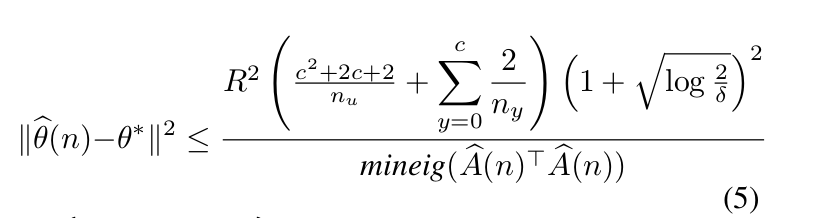
\includegraphics[bb=0 0 840 218,scale=0.3,keepaspectratio=true]{./bound.png}
 % bound.png: 840x218 pixel, 72dpi, 29.63x7.69 cm, bb=0 0 840 218
 \caption{Upper bound on the difference between the true class ratio and the predicted class ratio}
\end{figure}
The bound holds with probability atleast $\delta$, 
$n_y$ : Number of training instances, $n_u$ : Number of test instances, 
R is the data spread ($max_{x \in X}||\phi(x)||$), $c$ the number of classes


\end{frame}

\begin{frame}{MMD for Estimating Occurrence Statistics of Entities}
 \begin{alertblock}{Required}
 Given a corpus with mentions identified we want reliable estimates of frequency of each
of the entities.
\end{alertblock}
\begin{exampleblock}{Features}
Each mention has several candidate disambiguations. This gives one way of formulating the features. 
For each mention, we can have a (sparse) feature vector having non zero scores for the candidates.
\end{exampleblock}
\begin{exampleblock}{Training Data}

Can be obtained by splicing the named entity disambiguation pipeline of any of the popular
named entity disambiguators. [21] discusses how to achieve this for AIDA, a popular named entity
disambiguator.
\end{exampleblock}

\end{frame}
